\documentclass{beamer}

\usepackage[utf8]{inputenc}
\usepackage[russian]{babel}

\usepackage{graphicx}
\usepackage{gensymb}

\usefonttheme[onlymath]{serif}

%\usepackage{beamerthemesplit}
%\useoutertheme{infolines}
%\useoutertheme{smoothtree}
\useoutertheme{tree}
\useinnertheme{circles}
\setbeamertemplate{itemize items}[default]
\setbeamertemplate{enumerate items}[default]

\definecolor{myblue}{rgb}{.0,.2,.3}
\setbeamercolor*{palette primary}{use=structure,fg=white,bg=myblue}
\setbeamertemplate{navigation symbols}{}

\usepackage{tikz}
\usetikzlibrary{shapes.geometric, arrows, trees}
\tikzstyle{every node}=[font=\tiny, node distance=0.8cm]
\tikzstyle{io} = [trapezium, trapezium left angle=70, trapezium right angle=110, minimum width=1cm, minimum height=0.33cm, text centered, text width=1cm, draw=black, fill=blue!30]
\tikzstyle{process} = [rectangle, minimum width=1cm, minimum height=0.31cm, text centered, draw=black, fill=orange!30]
\tikzstyle{decision} = [diamond, minimum width=1cm, minimum height=0.31cm, text centered, draw=black, fill=green!30]
\tikzstyle{arrow} = [thick,->,>=stealth]
\tikzstyle{bigrect} = [rectangle, minimum width=5.5cm, minimum height=4.5cm, text depth=5cm, draw=black, dashed]

%\usepackage{verbatim}
\usepackage{listings}
%\usepackage{enumitem}
%\setlistdepth{9}
%\setlist[itemize,1]{label=$\bullet$}
%\setlist[itemize,2]{label=$\bullet$}
%\setlist[itemize,3]{label=$\bullet$}
%\setlist[itemize,4]{label=$\bullet$}
%\setlist[itemize,5]{label=$\bullet$}
%\setlist[itemize,6]{label=$\bullet$}
%\setlist[itemize,7]{label=$\bullet$}
%\setlist[itemize,8]{label=$\bullet$}
%\setlist[itemize,9]{label=$\bullet$}
%\renewlist{itemize}{itemize}{9}

\newcommand{\layersInRealLife} {
  \frametitle{Уровни (levels / layers) в реальной жизни}
  \framesubtitle{Уровни характеризуются \textbf{обязанностями} и определяют \textbf{кто над кем главнее (выше)}}

  \begin{itemize}
    \item Директор конторы (высокий уровень)
      \begin{itemize}
        \item Художник (низкий уровень)
        \item Программист (низкий уровень)
        \begin{itemize}
          \item Младший программист (самый низкий уровень)
        \end{itemize}
      \end{itemize}
  \end{itemize}
}

\newcommand{\paradigmsImpDecl} {
  \node (imper) [bigrect, xshift=-1cm] {Императивное};
  \node (decl) [bigrect, xshift=5cm, yshift=2.5cm] {Декларативное};
}

\newcommand{\paradigmsAlg} {
  \paradigmsImpDecl

  \node (alg) [process, dashed, xshift=-1cm, yshift=1cm] {Алгоритмическое};
    \node [xshift=-1cm, yshift=0.65cm] {Блок-схемы, словесное описание};
}

\newcommand{\paradigmsStruct} {
  \paradigmsAlg

  \node (struct) [process, xshift=0cm, yshift=0cm] {Структурное};
    \node [xshift=0cm, yshift=-0.35cm] {Ограничение алгоритмического};
  \draw [arrow] (alg) -- (struct);
}

\newcommand{\paradigmsProc} {
  \paradigmsStruct

  \node (proc) [process, xshift=-1cm, yshift=-1cm] {Процедурное};
    \node [xshift=-1cm, yshift=-1.35cm] {C, Pascal...};
  \draw [arrow] (struct) -- (proc);
}

\newcommand{\paradigmsOop} {
  \paradigmsProc

  \node (oop) [process, xshift=-1.5cm, yshift=-2cm] {Объектно-ориентированное (ООП)};
    \node [xshift=-1.5cm, yshift=-2.35cm] {C++, C\#, Java, Python, Ruby, JS, ...};
  \draw [arrow] (proc) -- (oop);
}

\newcommand{\paradigmsDecls} {
  \paradigmsOop

  \node (notprog) [process, dashed, xshift=5cm, yshift=4cm] {Описания};
    \node [xshift=5cm, yshift=3.65cm] {Конфигурации и Web API (XML, JSON),};
    \node [xshift=5cm, yshift=3.35cm] {вёрстка (HTML, LaTeX), аннотации};
}

\newcommand{\paradigmsFunc} {
  \paradigmsDecls

  \node (func) [process, xshift=4cm, yshift=2.5cm] {Функциональное};
}

\newcommand{\paradigmsLogical} {
  \paradigmsFunc

  \node (logical) [process, xshift=5cm, yshift=1cm] {Логическое};
}

\newcommand{\paradigmsAll} {
  \paradigmsLogical

  \node (generic) [process, xshift=-1cm, yshift=5cm] {Обобщенное};
  \node (concurrent) [process, xshift=5cm, yshift=-2cm] {Конкурентное};
  \node (module) [process, xshift=-2cm, yshift=4cm] {Модульное};
}


\title{Введение в программирование}
\author{Лопатин Александр}
\date{2015}


\subtitle{Лекция 2}

\begin{document}

  \frame{\titlepage}


  \section*{Содержание} {
    \frame{\tableofcontents[hideallsubsections]}


  \section{Языки программирования}
    \frame {
      \frametitle{Язык программирования}
      Знаковая система \underline{для написания компьютерных программ}

      \vspace{0.5cm}
      Текст, написанный на таком языке называют \underline{текст программы} или \underline{исходный~код}~(source~code) или просто \underline{код}
    }

    \frame {
      \frametitle{Трансляторы языков программирования}
      Программы, которые \underline{понимают исходный код}

      \vspace{0.5cm}
      Бывают двух типов:
      \begin{itemize}
        \item Компилятор --- превращает текст программы в \underline{двоичный код}
        \item Интерпретатор --- читает текст программы и выполняет написанное
      \end{itemize}
    }

    \frame {
      \frametitle{Двоичный код}
      \begin{itemize}
        \item \textbf{машинный код} (machine/native code) --- код, который исполняет \underline{аппаратный} исполнитель (например микропроцессор)
        \item \textbf{байт-код} \underline{виртуальной машины} --- код, который исполняет \underline{программный} исполнитель (например <<виртуальная машина .NET>> или <<виртуальная машина Java (JVM)>>) 
      \end{itemize}

      \vspace{0.5cm}
      Понятие <<виртуальная машина>> --- многозначно.
      Об этом разжевано здесь:
      \url{http://habrahabr.ru/company/intel/blog/254793/}
    }

    \frame {
      С ростом популярности \underline{JIT-компиляции} разделение \underline{трансляторов} на
      \underline{компиляторы} и \underline{интерпретаторы} не столь актуально

      \vspace{1cm}
      Большинство \underline{актуальных интерпретаторов} стало, грубо говоря,
      \underline{компиляторами} в \underline{машинный код})

      \vspace{1cm}
      \url{https://ru.wikipedia.org/wiki/JIT}
    }

    \frame {
      Лучше разделять сами языки (и то как их применяют), а не трансляторы:
      \begin{itemize}
        \item \textbf{Компилируемые} (Assembler, C++, C\#, Java, ...)
        \item \textbf{Скриптовые} (Python, Ruby, JavaScript/ECMAScript, bash/shell, cmd/bat, PowerShell, ...)
      \end{itemize}

      \vspace{0.5cm}
      Слово <<скриптовый>> всё же не имеет четкого значения и для многих является синонимом к интерпретируемым языкам

      \vspace{0.5cm}
      %\url{https://programmers.stackexchange.com/questions/46137/what-is-the-main-difference-between-scripting-languages-and-programming-language/46142\#46142}
      %\url{http://programmers.stackexchange.com/a/46142}
      \url{http://programmers.stackexchange.com/a/46233}
    }

    \frame {
      \frametitle{Компилируемые языки}
      Исходный код компилируют в \underline{двоичный код} и (обычно) распространяют в скомпилированном виде (.exe, .dll, .so и т.д.)

      \vspace{0.5cm}
      Часто используется для:
      \begin{itemize}
        \item \textbf{прикладного программирования} (от текстового редактора до веб-браузера или более сложной системы)
        \item \textbf{системного программирования} (драйвера устройств и т.д.)
      \end{itemize}

      \vspace{0.5cm}
      На них часто решают задачи, требующие высокой производительности
    }

    \frame {
      \frametitle{Скриптовые языки (языки сценариев)}
      \framesubtitle{Для многих --- синоним к <<Интерпретируемым языкам>>}
      Программы обычно распространяют в виде исходного кода (.py,~.js,~.bat~и~т.д.)

      \vspace{0.5cm}
      Часто используется для:
      \begin{itemize}
        \item \textbf{прототипов} прикладных программ
        \item \textbf{сценариев} для автоматизации задач, вроде сборка/тестирование/deploy билда
        \item написание пользовательских \textbf{макросов} для игры или электронной таблицы
        \item \textbf{плагинов/расширений} (для браузера, скажем)
        \item клиентский или серверный \textbf{код для веб-сайта}
      \end{itemize}

      \vspace{0.5cm}
      Популярно там, где хочется \underline{быстро увидеть результат}
    }

    \frame {
      А еще языки классифицируют по тому, на какие \textbf{парадигмы~программирования} сделан основной акцент...
    }

    \frame {
      \frametitle{Wait, wait...}
      \framesubtitle{Зачем об этом всём знать? --- Для осознания того}

      \begin{itemize}
        \item что языки можно \underline{очень по-разному} классифицировать
        \item \underline{одни классы} эффективно решают \underline{одни типы задач}, другие классы --- другие типы задач
        \item{} <<универсального>> языка \underline{не существует}
        \item чем более \underline{узкоспециализирован} язык (SQL для БД, G-Codes для станков, Verilog для спецификации устройств, GLSL для графики...) или комбинация языка и библиотеки/фреймворка (Ruby+RoR или JS+node.js для веб, ...) тем \underline{быстрее} их можно изучить
      \end{itemize}

      Другими словами --- чтобы появилось представление о \underline{способе выбора следующего языка} для изучения

      \vspace{0.5cm}
      \url{https://www.youtube.com/watch?v=LR8fQiskYII}
      \url{https://www.youtube.com/watch?v=NvWTnIoQZj4}
    }

    \frame {
      \frametitle{На википедии}
      Можно увидеть разницу между языками, если обращать внимание на \underline{Paradigm} и \underline{Typing discipline}
      \begin{center}
        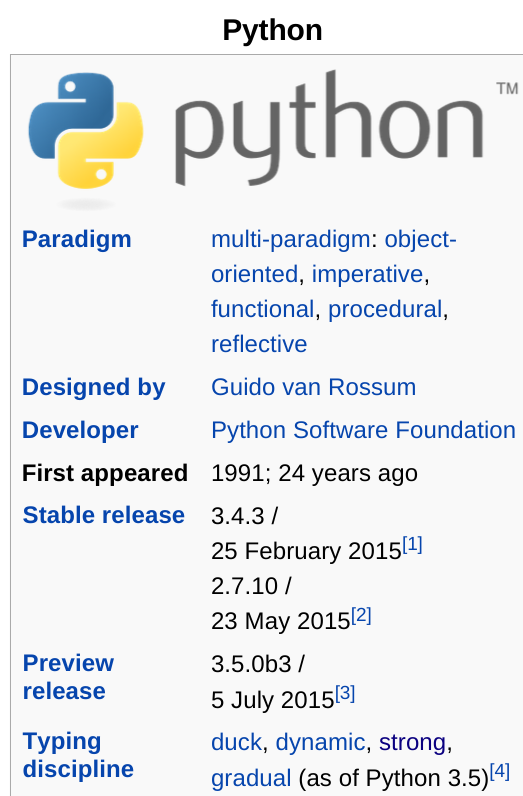
\includegraphics[scale=0.18]{pictures/python.png}
        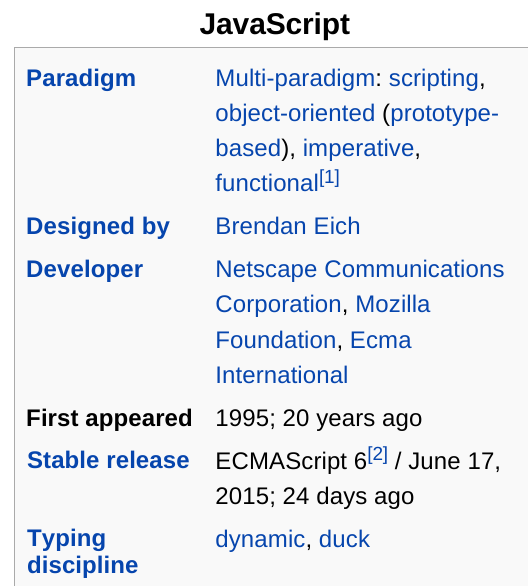
\includegraphics[scale=0.2]{pictures/js.png}
        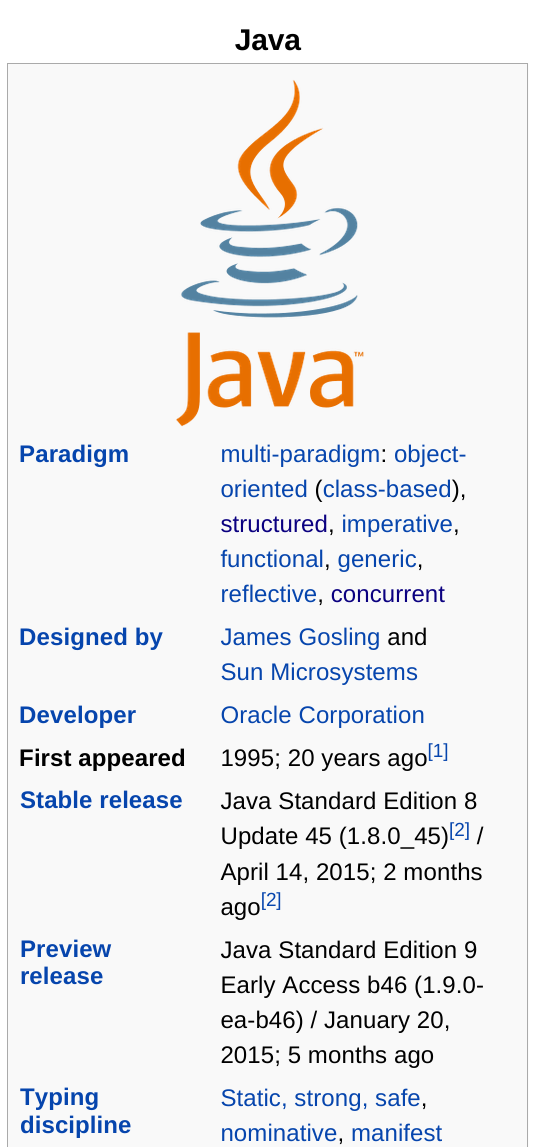
\includegraphics[scale=0.12]{pictures/java.png}
      \end{center}
    }

  \section{<<Hello world>> на всех языках}
\begin{frame}[fragile]
  \frametitle{Привет, Python 2!}
  \begin{minted}{python}
print "Hello World!"
  \end{minted}

  \vspace{2cm}
  Попробовать --- \url{http://tutorialspoint.com/execute\_python\_online.php}
\end{frame}

\begin{frame}[fragile]
  \frametitle{Привет, JavaScript (ECMAScript 6)!}
  \begin{minted}{js}
console.log("Hello World!")
  \end{minted}

  \vspace{1.5cm}
  Попробовать --- \url{http://www.es6fiddle.net/}
\end{frame}

\begin{frame}[fragile]
  \frametitle{Привет, Java 8!}
  \begin{minted}{java}
public class HelloWorld {
    public static void main(String[] args) {
        System.out.println("Hello World!");
    }
}
  \end{minted}

  \vspace{1.5cm}
  Попробовать --- %\url{http://www.tutorialspoint.com/compile\_java8\_online.php}
\url{http://www.compilejava.net/}
\end{frame}

\section{Переменные и константы}
\begin{frame}[fragile]
  \frametitle{Данные в языках --- это переменные и константы}
  \textbf{Переменную} можно изменять (время, координаты, ...)

  Пример на Java:
  \begin{minted}{java}
int x = 2;
System.out.println("x == " + x);       // x == 2
x = x + 1;
System.out.println("x == " + x);       // x == 3
  \end{minted}
  \vspace{1cm}
  \textbf{Константу} нельзя изменять (число $\pi$, скорость света ...)
  Пример на Java:
  \begin{minted}{java}
final double pi = 3.14;
  \end{minted}
\end{frame}

\frame {
  \frametitle{Данные могут быть разных типов}
  Примитивные (простые) типы:
  \begin{itemize}
    \item \textbf{целое} число (\underline{int}, long, ...): -123, 12345678910L
    \item \textbf{дробное} число (\underline{float}, double): 0.123f, 0.123
    \item \textbf{символ} (char): 'z'
  \end{itemize}

  \vspace{1cm}
  Составные типы:
  \begin{itemize}
    \item \textbf{массивы} (\underline{array}): [1, 2, 3, 4]
    \item \textbf{объекты} (\underline{string}, list, set, dict/map, ...): $"$Hello$"$, \{"hello":~"привет"\}
  \end{itemize}
}

\section{Действия (операторы)}
\begin{frame}[fragile]
  \frametitle{Присваивание (Python)}
  \begin{minted}{python}
x = 1
y = 2
print x       # 1
x = y
print x       # 2
x = y + 1
print x       # 3
  \end{minted}

  \vspace{0.5cm}
  Синтаксис: \underline{переменная = значение}

  Читается <<переменной присвоить значение>>

  \vspace{0.5cm}
  Или же: \underline{переменная = выражение}

  Читается <<переменной присвоить \underline{результат вычисления} выражения>>
\end{frame}

\begin{frame}[fragile]
  \frametitle{Арифметические операторы (Python)}
  \begin{minted}{python}
x = 2 + 2
print x               # 4
x = x - 1
print x               # 3
x = x * x
print x               # 9
print x % 2           # 1 (остаток от деления)
print x / 2           # 4 (целочисленное деление)
print x / 2.0         # 4.5 (деление целого на дробное)
print float(x) / 2.0  # 4.5
  \end{minted}
В предпоследнем: целое (int) было неявно преобразовано в дробное (float)
\end{frame}

\begin{frame}[fragile]
  \frametitle{Логические операторы (Python)}
  \begin{minted}{python}
x = True
y = False
print x and y        # False
print x or y         # True
print not x          # False (тоже самое, что и x == False)

a = 2
b = 3
print a < b          # True
print a > b          # False
print a <= b, a >= b # True False
print a == b         # False (читается "a равняется b")
print a == (b - 1)   # True
  \end{minted}
  Не путать \textbf{равенство} (логический оператор) с \textbf{присвоением} (действие, которое изменяет значение переменной)
\end{frame}

\begin{frame}[fragile]
  \frametitle{Логические операторы (JavaScript)}
  \begin{minted}{js}
var x = true
var y = false
console.log(x && y)    // false
console.log(x || y)    // true
console.log(!x)        // false

var a = 2
var b = 3
// операторы сравнения везде одинаковые, кроме равенства
console.log(a === b)   // false
  \end{minted}
\end{frame}

\begin{frame}[fragile]
  \underline{Порядок вычислений} зависит от \underline{приоритетов операторов}

  Например в выражении
  \begin{minted}{python}
y = a + b * c
  \end{minted}
  сначала будет выполнено умножение, потом --- сложение.
\end{frame}

\begin{frame}[fragile]
  На \underline{порядок вычислений} можно повлиять, расставив \underline{скобки}
  \begin{minted}{python}
y = (a + b) * c
  \end{minted}

\vspace{0.5cm}
Существуют операторы, которые имеют разные приоритеты, \underline{в зависимости от языка}

\vspace{0.5cm}
В случае неуверенности в порядке вычислений --- нужно проставлять скобки
\end{frame}

\begin{frame}[fragile]
  А в случае со \underline{слишком длинным} выражением --- лучше \underline{распилить} его на части

  \vspace{0.5cm}
  Например вместо
  \begin{minted}{python}
pageHeight = headerHeight + itemHeight * newsNumber +
             footerHeight
  \end{minted}

\vspace{0.5cm}
написать что-то вроде
  \begin{minted}{python}
newsHeight = itemHeight * newsNumber
pageHeight = headerHeight + newsHeight + footerHeight
  \end{minted}
\end{frame}

\begin{frame}[fragile]
  \frametitle{Ввод (Python)}
  \begin{minted}{python}
line = raw_input("input a number: ") # ввод строки
number = int(line)                   # преобр. в целое
line = raw_input("input something: ")# снова ввод строки
floatNumber = float(line)            # преобр.
                                     # в дробное
  \end{minted}
\end{frame}

\begin{frame}[fragile]
  \frametitle{Массивы (Python)}
  \begin{minted}{python}
x = [1, 2, 55, -123]
i = 2
print x[i]            # 55
x[i] = 777
print x               # [1, 2, 777, -55]
n = len(x)
print n               # 4
  \end{minted}

  \vspace{0.5cm}
  n --- это \textbf{размер} или \textbf{длина} массива

  i --- это \textbf{индекс} массива

  Индексация (обычно) начинается с нуля
\end{frame}

\begin{frame}[fragile]
  \frametitle{Массивы (Java)}
  \begin{minted}{java}
int x[] = {1, 2, 55, -123};
int y[] = new int[x.length];
System.out.println("length is " + x.length);
// length is 4
  \end{minted}

  \vspace{0.5cm}
  Подробней --- \url{http://www.tutorialspoint.com/java/java\_arrays.htm}
\end{frame}

\begin{frame}[fragile]
  \frametitle{Массивы (JavaScript)}
  \begin{minted}{js}
var x = [1, 2, 55, -123]
// индексировать, изменять и получать размер
// - как в Java
  \end{minted}

  \vspace{0.5cm}
  Подробней --- \url{http://www.w3schools.com/js/js\_arrays.asp}
\end{frame}

\begin{frame}[fragile]
  \frametitle{Массивы могут быть вложены}
  Массивы с двумя уровнями вложенности называют \underline{двумерными} или
  <<массив \underline{размерности} два>>

  (не путать с \underline{размерность} с \underline{размером})

  \vspace{0.5cm}
  Пример (на Python) массива 2x4 (размерности 2, размера 4; или с 2-мя \underline{строками} и 4-мя \underline{столбцами}):
  \begin{minted}{python}
x = [[1, 2, 55, -123], [4, 5, 6, 7]]
x[1][3] = 4444
print x
[[1, 2, 55, -123], [4, 5, 6, 4444]]
  \end{minted}
\end{frame}

\begin{frame}[fragile]
  \frametitle{Ввод (Java)}
  \begin{minted}{java}
import java.util.Scanner;            // импорт библиотеки
...
Scanner in = new Scanner(System.in); // создание объекта
String line = in.nextLine();         // получение строки
int number = in.nextInt();           // получение целого
float floatNumber = in.nextFloat();  // получение дробного
  \end{minted}
\end{frame}

\frame {
  \frametitle{Ввод (JavaScript)}
  Там для этого можно использовать HTML-форму

  \vspace{0.5cm}
  Пока не будем это использовать
}

\frame {
  \frametitle{Практика}

  Поиграться с описанным выше на всех языках
}

\section{Структурное программирование}
\begin{frame}[fragile]
\frametitle{Условия (JavaScript)}
\begin{columns}
  \column{0.5\textwidth}
    \begin{minted}{js}
var a = true
var b = false

// с одной веткой
if (a && b) {
  console.log("both are true")
}
    \end{minted}
  \column{0.5\textwidth}
    \begin{minted}{js}
// с двумя ветками
if (a && b) {
  console.log("both are true")
} else {
  console.log("one of them")
}
    \end{minted}
  \end{columns}
\end{frame}

\begin{frame}[fragile]
\frametitle{Вложенные условия (JavaScript)}
\begin{columns}
  \column{0.5\textwidth}
    \begin{minted}{js}
var a = true
var b = false

if (a && b) {
  console.log("both are true")
} else {
  if (!a) {
    console.log("a is false")
  } else {
    console.log("b is false")
  }
}
    \end{minted}
  \column{0.5\textwidth}
    \begin{minted}{js}
// более читаемый вариант
if (a && b) {
  console.log("both are true")
} else if (!a) {
  console.log("a is false")
} else {
  console.log("b is false")
}
    \end{minted}
  \end{columns}
  Hint: надо всегда выделять ветки условий в фигурные скобки в языках JS и Java
\end{frame}

\begin{frame}[fragile]
\frametitle{Вложенные условия (Python)}
  \begin{minted}{python}
a = True
b = False

if a and b:
    print "both are true"
elif not a:
    print "a is false"
else:
    print "b is false"
  \end{minted}
\end{frame}

\begin{frame}[fragile]
\frametitle{Цикл с предусловием (Python)}
  \begin{minted}{python}
i = 0
while i < 10:
    print i
    i = i + 1
  \end{minted}
\end{frame}

\begin{frame}[fragile]
  \frametitle{Цикл с постусловием (Java)}
  \begin{minted}{java}
int i = 0;
do {
    System.out.println("i = " + i)
    i = i + 1;
} while (i < 10);
  \end{minted}
\end{frame}


\begin{frame}[fragile]
  \frametitle{Эмуляция цикла с постусловием (Python)}
  \framesubtitle{Настоящего цикла с постусловием в Python нет}
  \begin{minted}{python}
i = 0
conditionMet = False
while not condMet:
    print "i =", i
    i = i + 1
    if i < 10:
        condMet = True
  \end{minted}
\end{frame}

\begin{frame}[fragile]
  \frametitle{Цикл со счетчиком (Java)}
  \begin{minted}{java}
for (int i = 0; i < 10; i = i + 1) {
    System.out.println("i = " + i)
}
  \end{minted}
\end{frame}

\begin{frame}[fragile]
  \frametitle{Цикл со <<счетчиком>> (Python)}
  \begin{minted}{python}
for i in range(0, 10, 1):
    print "i = " + str(i)
  \end{minted}
\end{frame}

\begin{frame}[fragile]
  \frametitle{Циклы могут быть вложены (Python)}
  \begin{minted}{python}
a = [[4, 5, 6], [7, 8, 9]]
n = len(a)
m = len(a[0])

for i in range(0, 2, 1):
    j = 0
    while j < m:
        print "i =", i, " j =", j
        print a[i][j]
        j = j + 1
  \end{minted}
\end{frame}

    \frame {
      \frametitle{Практика}

      Поиграться с описанным выше на всех языках

      \vspace{0.5cm}
      Написать примитивный калькулятор

      \vspace{0.5cm}
      Написать алгоритм поиска наибольшего элемента в одномерном массиве
    }

    \frame {
      \frametitle{Домашка}

      На \underline{любом} из трёх языков программирования: Python, JavaScript или Java (по +1 баллу за реализацию на других языках, из перечисленных):

        \begin{enumerate}
          \item Реализовать задачу из предыдущей лекции (решение квадратного уравнения)
          \item Дан одномерный массив из $n$ целочисленных элементов (реализовывать ввод массива не нужно). Инвертировать порядок элементов в этом массиве
          \item Бонусная задача: дан двумерный массив целочисленных элементов (реализовывать ввод массива не нужно) из $n$ строк и $m$ столбцов. Вывести \underline{номер строки} и \underline{столбца} \underline{наименьшего элемента}
            \begin{itemize}
                \item подсказка: стоит начать с упрощенной версии программы: вывод наименьшего \underline{элемента} \underline{одномерного} массива, усложнить до вывода \underline{индекса} наименьшего элемента \underline{одномерного} массива и только потом пытаться реализовать тоже самое для двумерного массива
            \end{itemize}
        \end{enumerate}
    }
\end{document}
